\subsubsection*{AML}

\paragraph{Overview}

AML is a memory management library designed to ease the use of complex
memory topologies and complex data layout optimizations for
HPC applications.

AML is a framework providing locality-preserving abstractions to
application developers.  In particular, AML aims to expose flexible
interfaces to describe and reason about how applications deal with data
layout, tiling of data, placement of data across hardware topologies, and
affinity between work and data.

\paragraph{Key Challenges}

Between non-uniform memory access (NUMA) to regular DRAM, the 3-D stacked
high-bandwidth memory, and the memory local to the accelerator devices such
as GPUs, the increasing depth of the memory hierarchy presents exascale
applications with a critical challenge of how to use the available
heterogeneous memory resources effectively.

Standardized interfaces to manage complex memory hierarchies are lacking,
and vendors are reluctant to innovate in this space in the absence of clear
directions from the community.  Coming up with an interface that is
sufficiently expressive to cover the emerging and projected hardware
advances, yet is simple enough and practical to be both acceptable and
useful to the applications is the key challenge that we are working on
addressing.

\paragraph{Solution Strategy}

AML provides explicit, application-aware memory management for deep memory
systems.  It offers a collection of building blocks that
are \emph{generic}, \emph{customizable}, and \emph{composable}.
Applications can specialize the implementation of each offered abstraction
and can mix and match the components as needed.  AML building blocks can be
used to create, for example, mechanisms to replicate data across memory
devices. We provide some high-level interfaces, built on top of these
building blocks, as examples of what can be done with AML and as features
more readily usable by applications. 

We provide applications and runtimes with a descriptive API for data
access, where all data placement decisions are explicit, and so is the
movement of data between different memory types.  At the same time, the API
does abstract the memory topology and other device complexities.  We focus
on optimizing data locality for current and future hardware generations;
applications provide insights for static allocations, and we can also
dynamically and asynchronously move or transform data to optimize for a particular 
device or to best take advantage of the memory hierarchy.

\begin{wrapfigure}[6]{r}{.18\textwidth}
%\vspace{-12pt}%
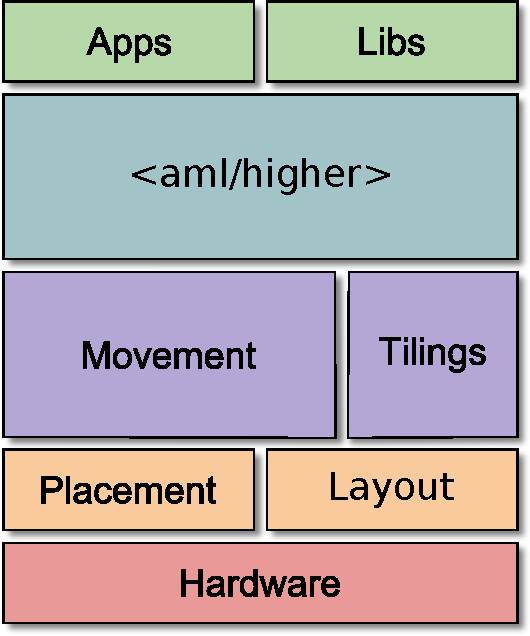
\includegraphics[width=.18\textwidth]{projects/2.3.1-PMR/2.3.1.19-Argo-PowerSteering/aml-components}
\end{wrapfigure}
AML components are built on top of hardware drivers and system
libraries (libnuma, hwloc, accelerator libraries, other ECP products).
The figure on the right depicts the major components of AML, including:
\begin{itemize}
\item Placement: mechanisms to decide where data lives,
\item Layout: descriptions of the shape of applications data,
\item Movement: how to move data across devices (including transformations),
\item Tiling: how to iterate over and generate collections of data chunks,
\item High level abstractions and helpers.
\end{itemize}

\paragraph{Recent Progress}

This year AML contributions are distributed between new features and
support for new devices.

As part of our effort to offer AML as a framework to abstract over many
different types of heterogeneous memory devices, we implemented support for
two more vendor APIs: OpenCL and Intel oneAPI (through Level Zero). This
support allows application users to use AML on more platforms, while still
offering the same level of portability as with the rest of the AML code:
even though the initialization of a specific implementation of a building
block is unique to that implementation, the code that makes use of this
building block is generic across implementations. This design choice should
keep application modifications at a reasonable level.

As we extend support for new devices in AML, the core abstractions offered
by the library might end up being challenged by small differences in the
low-level driver interfaces we support. This year, these challenges
resulted in data movement facilities in AML receiving major improvements,
in particular with respect to creating batches of requests to move small
chunks of data. AML can now avoid creating request objects when many
requests need to be performed at once, lowering the overhead of these types
of movement.

Furthermore, we developed for our ExaSMR collaborators a new feature
inspired by OpenMP 5 \emph{custom mappers}. An OpenMP mapper makes it
possible to describe which parts of a structure should be mapped onto
accelerator devices. As it is a recent addition to the standard, it is
currently poorly supported by compilers and lacks many features. For
example, its current design is limited in its ability to filter or
reorganize memory during the mapping process. We are using our
\emph{tiling} abstraction to build a more flexible interface for such a
feature.    Finally, we recently introduced in the library a new facility
to create custom allocators, on top of our placement building block
(areas). These custom allocators offer a similar interface to the standard
malloc/free C APIs, but allow for customization of the algorithm used to
manage chunks of free memory. For example, we offer allocators that don't
release memory to the devices on \texttt{free}, instead keeping it for
future allocation requests, or allocators that always use the same chunk
size for all requests. This new allocator facility should improve the
performance and flexibility of applications with specific use cases (e.g.,
many temporary allocations).

\paragraph{Preliminary Experiences on Early Access Systems}

The latest AML release (0.2.0) includes support for Intel oneAPI and AMD
HIP, which enables its use across CPUs and GPUs of Early Access Systems at
ALCF and OLCF.  We have successfully compiled it on the Spock system
(Frontier EAS) at OLCF and we verified that the testsuite completed
successfully.

\paragraph{Next Steps}

In a past collaboration with the author of the XSBench application, we
demonstrated a consistent speedup across a variety of shared memory systems
using the AML replicaset abstraction. As depicted in the figure below, we were
able to outperform or match existing solutions involving OpenMP or MPI by
using this abstraction. Since the previous iteration of this report, we
also implemented the mapper abstraction described above. We are planning to
continue this collaboration to implement a versatile replicaset abstraction
using the aforementioned mapper in order to duplicate complex data
structures in low-latency memories. The goal is to accelerate OpenMC
application while minimizing changes in the original code.
\begin{figure}[htb]
\centering
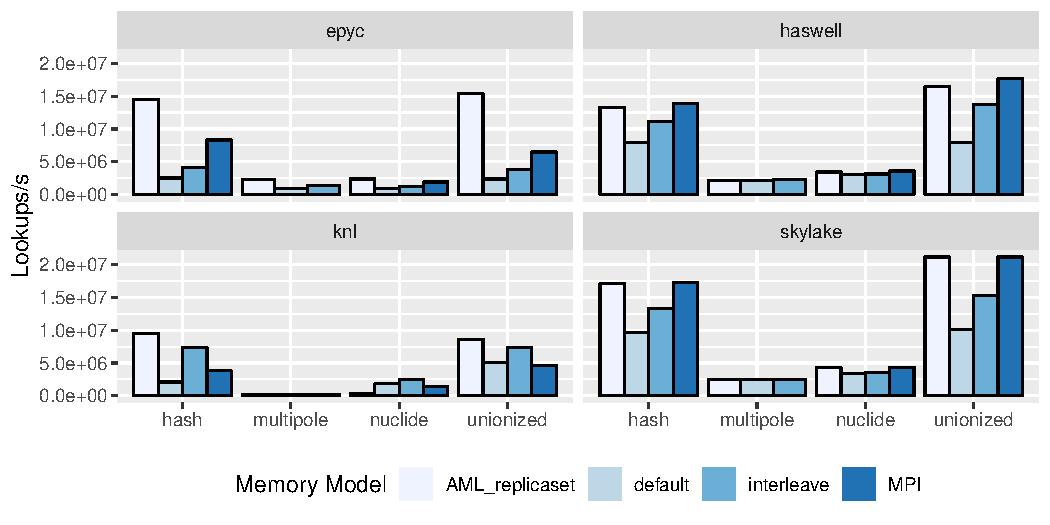
\includegraphics[width=.8\textwidth]{projects/2.3.1-PMR/2.3.1.19-Argo-PowerSteering/aml-xsbench}
\caption{Performance of AML replicaset on different hardware
architectures}
\end{figure}

We will continue to improve on our mapper facility based on the feedback
from the ExaSMR developers. In particular, we are looking to split this
feature into two interacting but independent components: a facility to
describe how collections of complex application data structures are
organized in memory, and a facility to navigate such data structures to
transform and map them into a separate virtual memory region. Our goal is
to improve the flexibility of our mapper to allow for more optimizations in
the number of data movements and data allocations when data is moved
between devices. A flexible enough mapper should also allow us to perform
an optimization similar to the replicaset: replicating subsets of the
memory being mapped on different memories to improve application
performance.
